\documentclass{beamer}
\usepackage{xeCJK}
\usepackage{graphicx}
\usepackage{float}
\usepackage{subfigure}

\usetheme{CambridgeUS}

\title{广州酒店的暖通设计}
\subtitle{毕业设计开题报告}
\author{郑海腾}
\institute{宁波工程学院}
\date{\today}

\begin{document}

\frame{\titlepage}

\section{外文翻译}
\begin{frame}

\begin{figure}[h]
\centering  %图片全局居中
\subfigure{
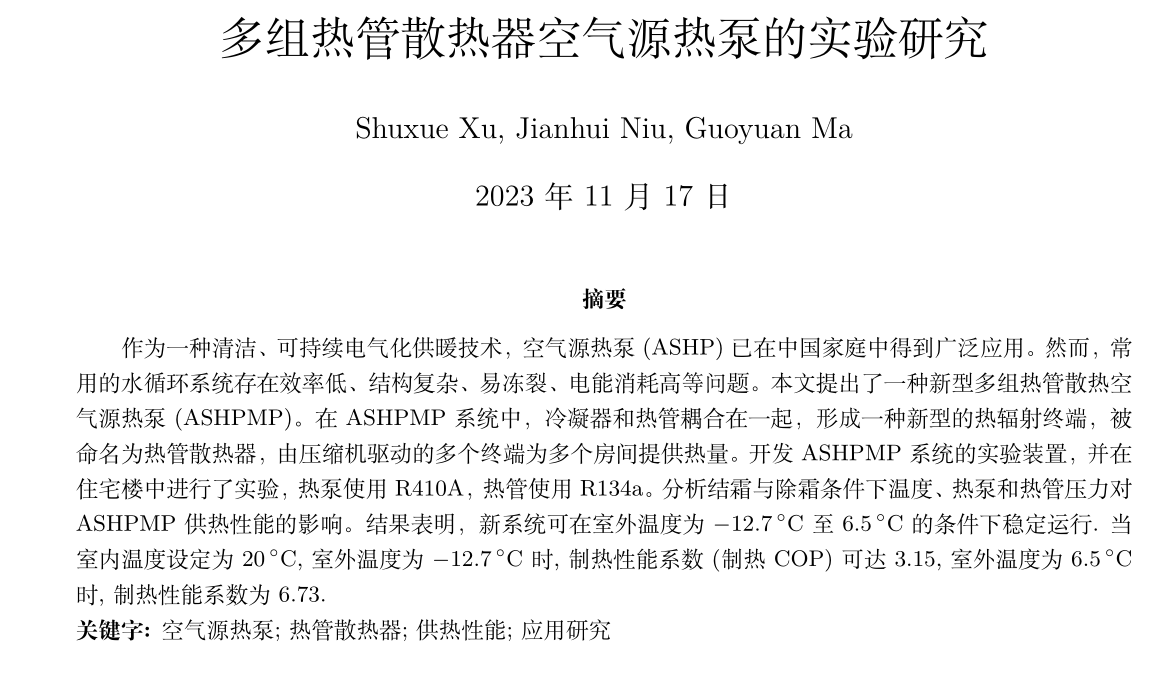
\includegraphics[width=0.5\textwidth]{figure_1}}
\subfigure{
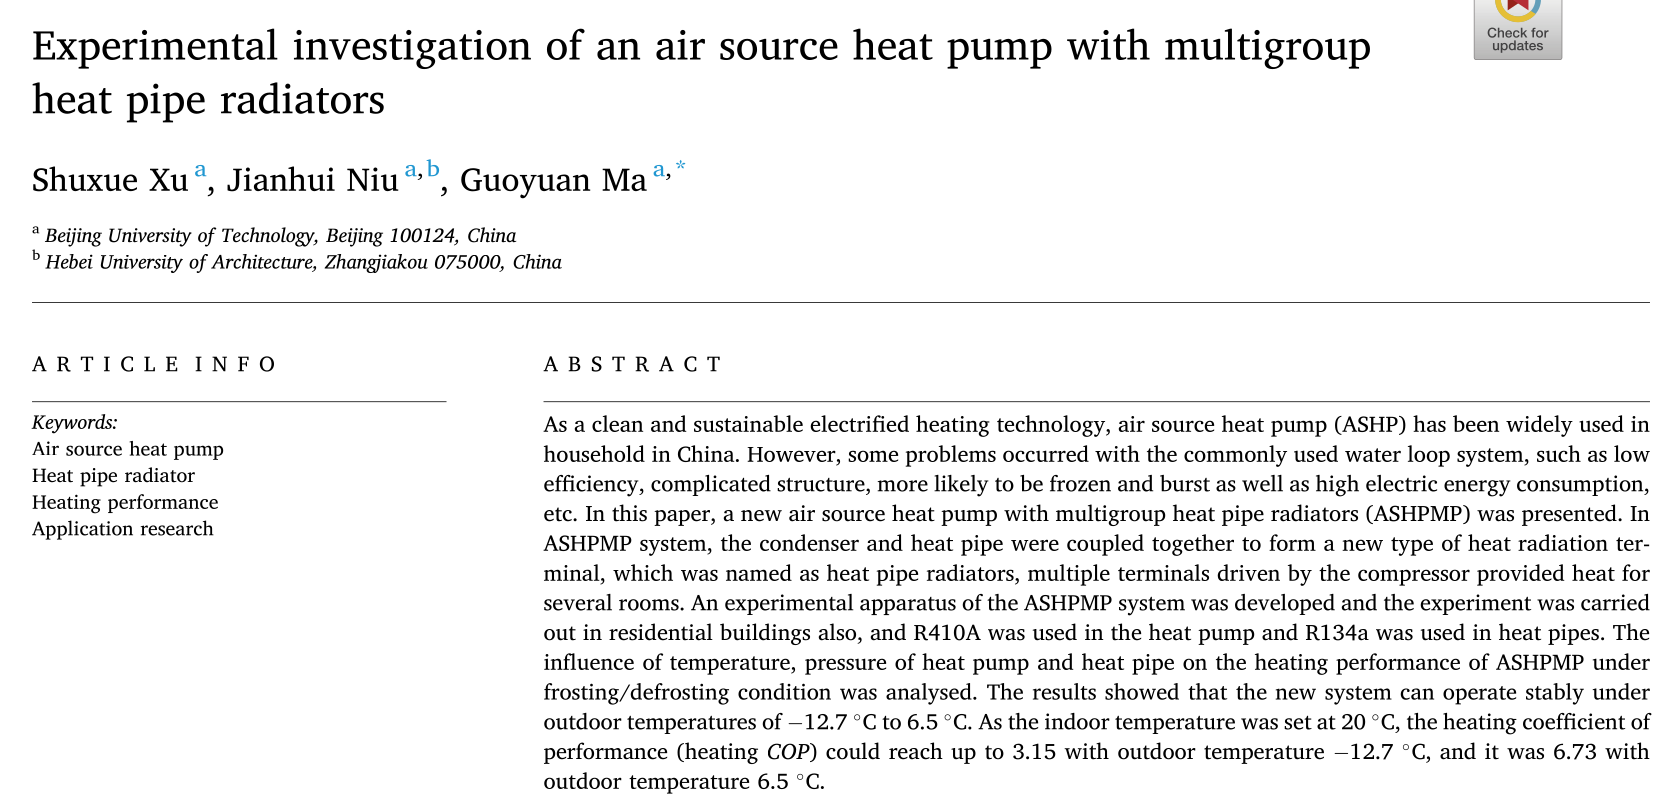
\includegraphics[width=0.5\textwidth]{figure_3}}
\end{figure}

\end{frame}

\begin{frame}

\begin{figure}[h]
\centering  %图片全局居中
\subfigure{
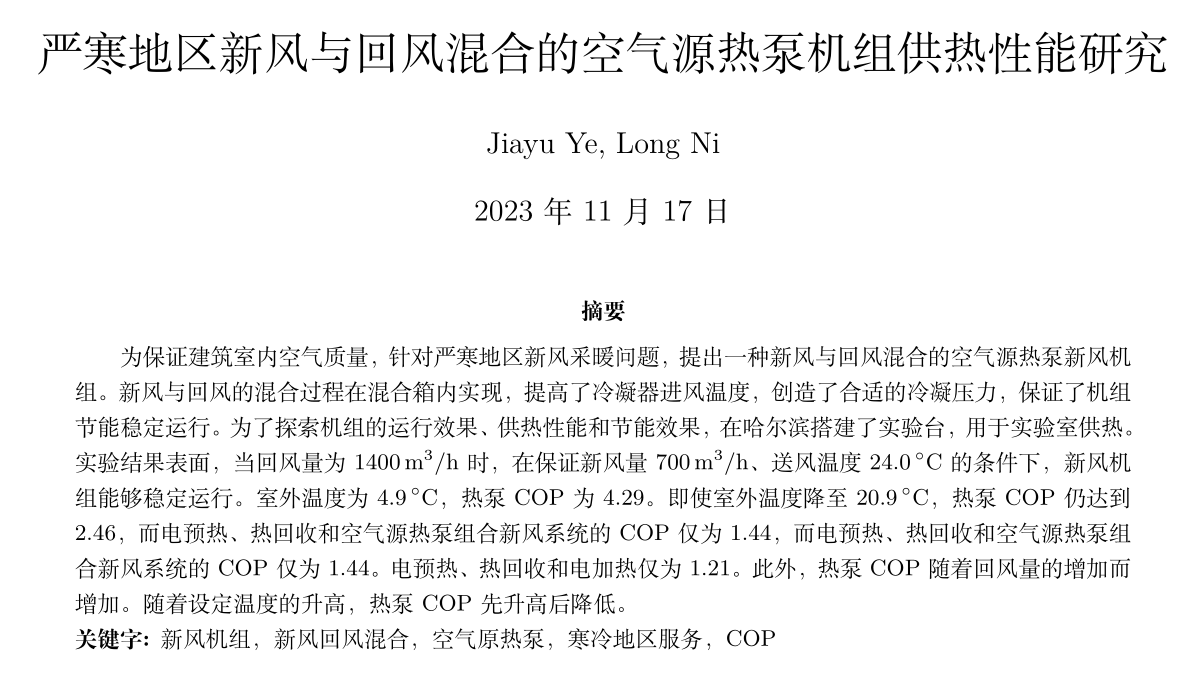
\includegraphics[width=0.5\textwidth]{figure_2}}
\subfigure{
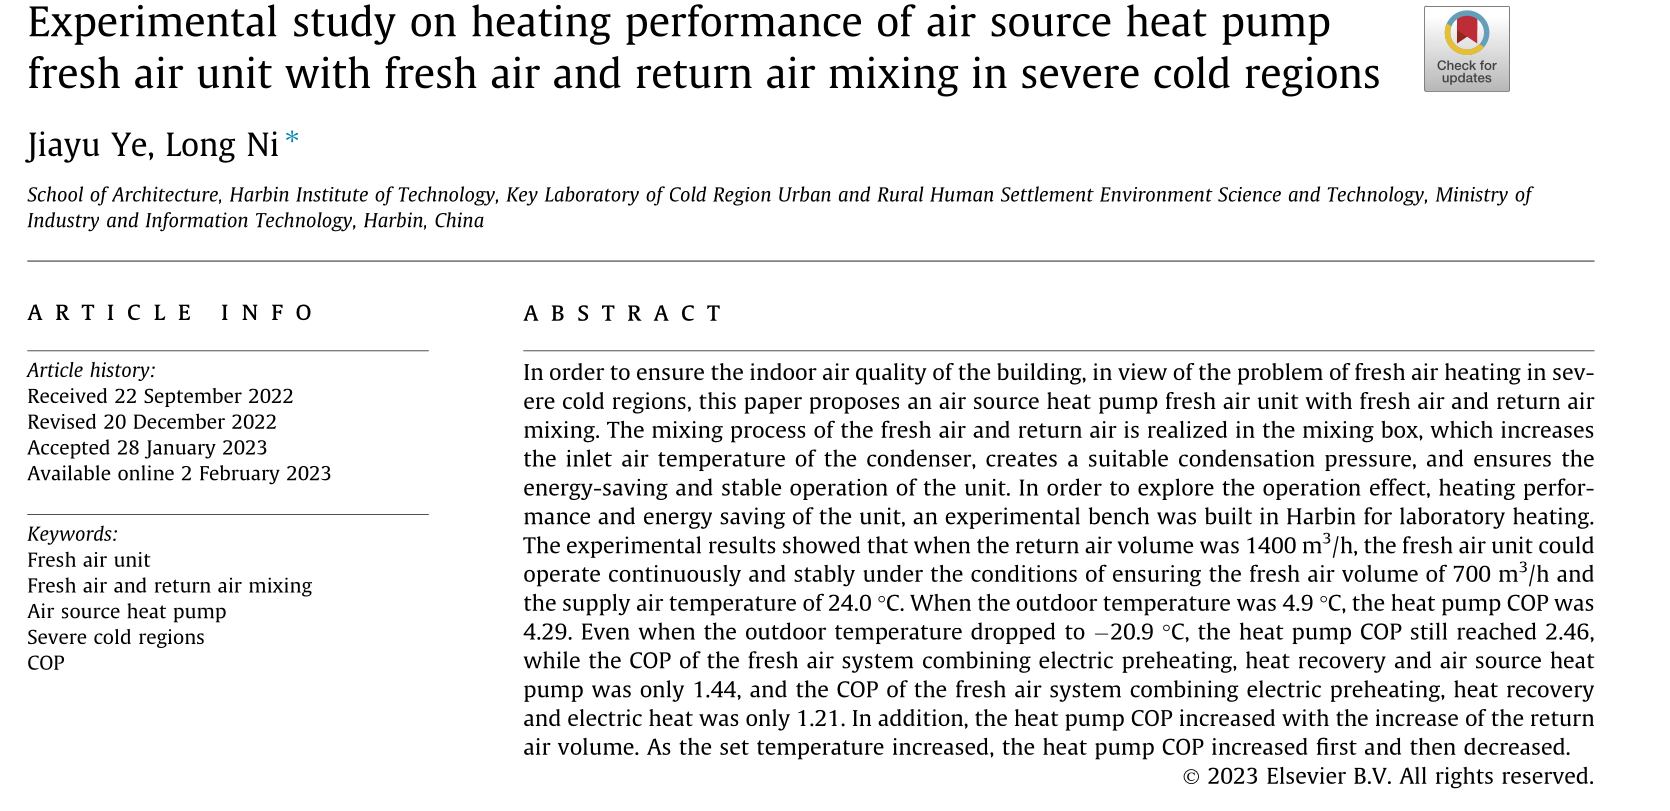
\includegraphics[width=0.5\textwidth]{figure_4}}
\end{figure}
	
\end{frame}

\section{工程概况}
\begin{frame}
	\begin{figure}[htbp]
	\centering
	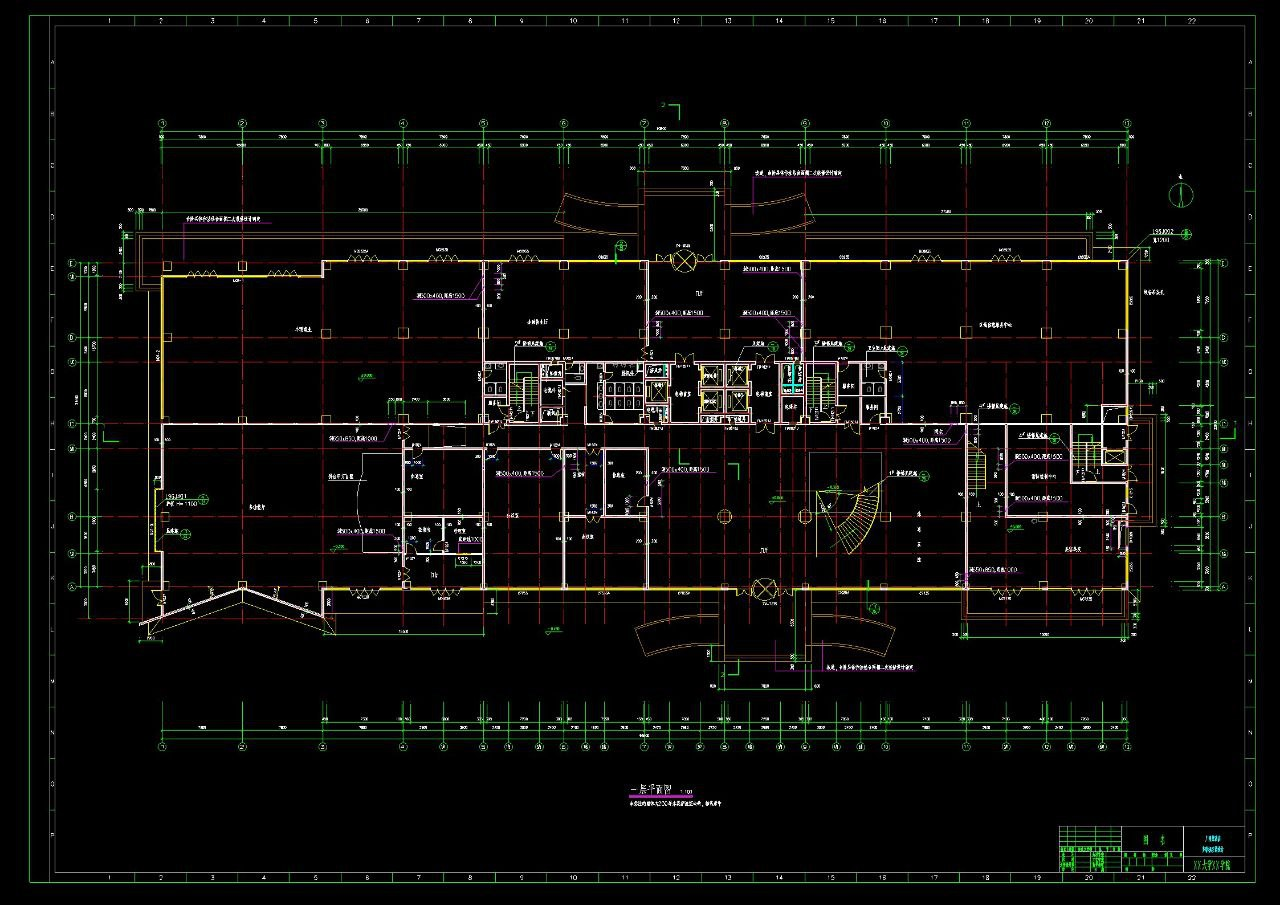
\includegraphics[width=0.7\textwidth]{figure_5}
	\end{figure}
\end{frame}

\begin{frame}
	该工程为 13 层高层建筑。该酒店包含休息室、接待室、控制室、大厅、会厅和客房等部分。大致长 96 米,宽 32 米。
	设计思路:客房等独立小房间采用风机盘管 + 新风系统。新风系统采用分楼层水平送风。广州地理位置靠南,夏热冬暖,采用风冷式机组。
\end{frame}

\section{文献综述}
\begin{frame}
	\begin{figure}[htbp]
	\centering
	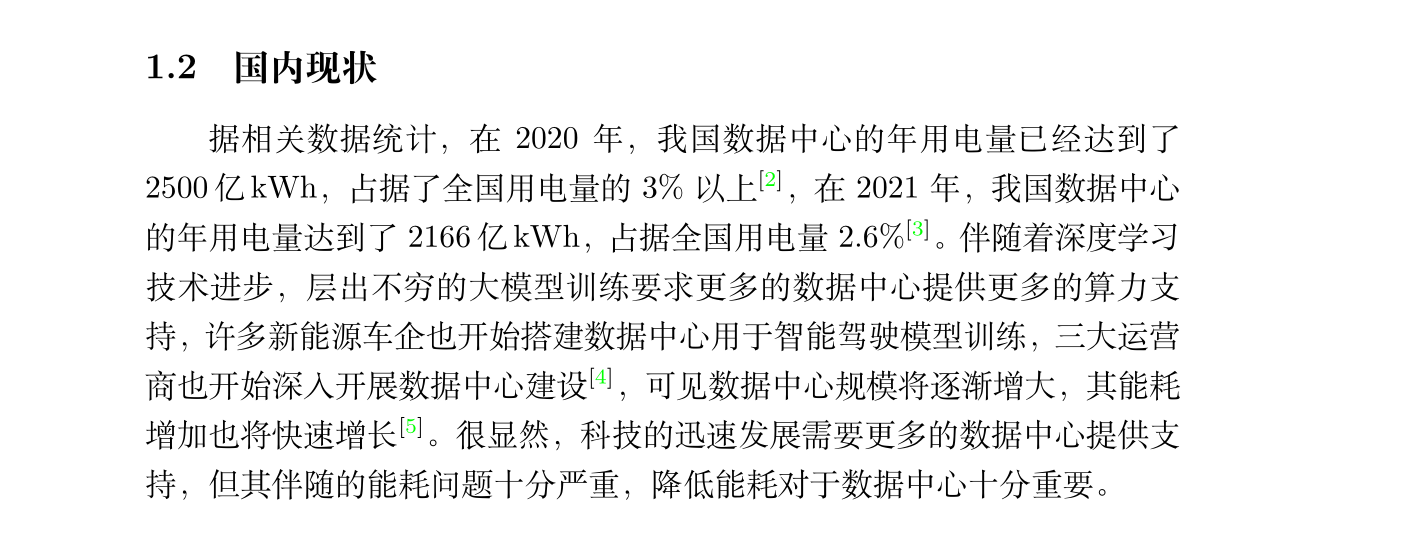
\includegraphics[width=0.7\textwidth]{figure_6}
	\end{figure}
	研究主题:数据中心的气流组织。
\end{frame}

\begin{frame}
	在计算机技术快速发展的今天,数据中心的数量也随着巨大的市场需求逐步增加。由于数据中心的能耗较大,因此探究其节能问题十分重要。空气中的气流组织对数据中心的能耗有影响。本文献综合探究了气流组织的特点与影响。
\end{frame}

\end{document}
